\documentclass[aspectratio=169]{beamer}

\usetheme{Boadilla}
\usefonttheme{professionalfonts}
\setbeamertemplate{navigation symbols}{}
\setbeamertemplate{itemize items}[circle]
\setbeamertemplate{enumerate items}[default]
\setbeamertemplate{headline}{}

\usepackage[utf8]{inputenc}
\usepackage[T1]{fontenc}
\usepackage{lmodern}
\usepackage{amsmath}
\usepackage{booktabs}
\usepackage{tabularx}
\usepackage{array}
\usepackage{hyperref}
\usepackage[strings]{underscore}
\usepackage{listings}
\usepackage{tikz}
\usetikzlibrary{arrows.meta,positioning,fit,calc,shapes.geometric}
\usepackage{xcolor}

\definecolor{courseblue}{HTML}{12355B}
\definecolor{coursegold}{HTML}{C98A2E}
\definecolor{courseice}{HTML}{EEF3F8}
\definecolor{coursegreen}{HTML}{2F6B4F}
\definecolor{coursegray}{HTML}{4B5563}
\definecolor{codebg}{HTML}{F7F9FC}
\definecolor{codecomment}{HTML}{5E6C84}
\definecolor{codestring}{HTML}{0B6E4F}

\setbeamercolor{palette primary}{bg=courseblue,fg=white}
\setbeamercolor{palette secondary}{bg=coursegold,fg=white}
\setbeamercolor{palette tertiary}{bg=courseblue,fg=white}
\setbeamercolor{palette quaternary}{bg=coursegold,fg=white}
\setbeamercolor{structure}{fg=courseblue}
\setbeamercolor{frametitle}{bg=courseice,fg=courseblue}
\setbeamercolor{title}{fg=courseblue}
\setbeamercolor{block title}{bg=courseblue,fg=white}
\setbeamercolor{block body}{bg=courseice,fg=black}
\setbeamercolor{normal text}{fg=black,bg=white}
\setbeamercolor{alerted text}{fg=coursegold}

\setbeamerfont{footline}{size=\scriptsize}

\setbeamertemplate{footline}{
  \leavevmode
  \hbox{
    \begin{beamercolorbox}[wd=.33\paperwidth,ht=2.8ex,dp=1.2ex,leftskip=0.8em]{palette primary}%
      University of Trieste
    \end{beamercolorbox}%
    \begin{beamercolorbox}[wd=.49\paperwidth,ht=2.8ex,dp=1.2ex,center]{palette tertiary}%
      \coursename{} \textbar{} \coursecode
    \end{beamercolorbox}%
    \begin{beamercolorbox}[wd=.18\paperwidth,ht=2.8ex,dp=1.2ex,right,rightskip=0.8em]{palette secondary}%
      \insertframenumber{} / \inserttotalframenumber
    \end{beamercolorbox}%
  }
}

\hypersetup{
  colorlinks=true,
  linkcolor=courseblue,
  urlcolor=coursegreen
}

\lstdefinestyle{coursepython}{
  language=Python,
  basicstyle=\ttfamily\footnotesize,
  keywordstyle=\color{courseblue}\bfseries,
  commentstyle=\color{codecomment}\itshape,
  stringstyle=\color{codestring},
  showstringspaces=false,
  columns=fullflexible,
  keepspaces=true,
  frame=single,
  framerule=0.6pt,
  rulecolor=\color{courseblue},
  backgroundcolor=\color{codebg},
  xleftmargin=0.4em,
  xrightmargin=0.4em,
  aboveskip=0.4em,
  belowskip=0.2em
}

\newcommand{\coursename}{Data-driven Systems Engineering}
\newcommand{\coursecode}{440MI / 305SM}
\newcommand{\coursefooter}{}

\newcommand{\learninggoals}[1]{
  \begin{block}{Learning goals}
  #1
  \end{block}
}

\newcommand{\repoactivity}[1]{
  \begin{block}{Repo activity}
  #1
  \end{block}
}

\newcommand{\readinglist}[1]{
  \begin{block}{Papers and materials}
  {\footnotesize #1}
  \end{block}
}

\newcommand{\coursecontextframe}[5]{
  \begin{frame}{Course Map and Running Cases}
  \centering
  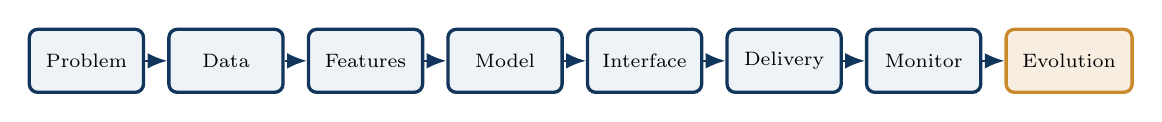
\begin{tikzpicture}[node distance=0.28cm]
  \node[flowbox, minimum width=1.45cm, minimum height=0.8cm] (problem) {\scriptsize Problem};
  \node[flowbox, minimum width=1.45cm, minimum height=0.8cm, right=of problem] (data) {\scriptsize Data};
  \node[flowbox, minimum width=1.45cm, minimum height=0.8cm, right=of data] (features) {\scriptsize Features};
  \node[flowbox, minimum width=1.45cm, minimum height=0.8cm, right=of features] (model) {\scriptsize Model};
  \node[flowbox, minimum width=1.45cm, minimum height=0.8cm, right=of model] (interface) {\scriptsize Interface};
  \node[flowbox, minimum width=1.45cm, minimum height=0.8cm, right=of interface] (delivery) {\scriptsize Delivery};
  \node[flowbox, minimum width=1.45cm, minimum height=0.8cm, right=of delivery] (monitor) {\scriptsize Monitor};
  \node[accentbox, minimum width=1.6cm, minimum height=0.8cm, right=of monitor] (evolution) {\scriptsize Evolution};
  \foreach \a/\b in {problem/data,data/features,features/model,model/interface,interface/delivery,delivery/monitor,monitor/evolution} {
    \draw[arrow] (\a) -- (\b);
  }
  \end{tikzpicture}

  \vspace{0.5em}
  \begin{block}{Today in the course}
  \textbf{Focus:} #1

  \textbf{Bridge:} #2
  \end{block}

  \begin{columns}[T]
  \column{0.48\textwidth}
  \begin{block}{Fraud case}
  {\footnotesize #3}
  \end{block}
  \column{0.48\textwidth}
  \begin{block}{Pasteurization case}
  {\footnotesize #4}
  \end{block}
  \end{columns}

  \vspace{0.3em}
  {\footnotesize \textbf{Course thread:} #5}
  \coursefooter
  \end{frame}
}

\newcommand{\classclosingframe}[4]{
  \begin{frame}{From This Class to the Next}
  \begin{block}{What stays with us}
  #1
  \end{block}

  \begin{columns}[T]
  \column{0.48\textwidth}
  \begin{block}{Project use}
  {\footnotesize #2}
  \end{block}
  \column{0.48\textwidth}
  \begin{block}{Next connection}
  {\footnotesize #3}
  \end{block}
  \end{columns}

  \vspace{0.3em}
  {\footnotesize \textbf{Course thread:} #4}
  \coursefooter
  \end{frame}
}

\tikzset{
  flowbox/.style={
    rounded corners=3pt,
    draw=courseblue,
    fill=courseice,
    very thick,
    minimum width=2.2cm,
    minimum height=0.9cm,
    align=center,
    font=\small
  },
  accentbox/.style={
    rounded corners=3pt,
    draw=coursegold,
    fill=coursegold!15,
    very thick,
    minimum width=2.2cm,
    minimum height=0.9cm,
    align=center,
    font=\small
  },
  arrow/.style={
    -{Latex[length=2.5mm,width=2mm]},
    thick,
    draw=courseblue
  }
}

\usepackage{amssymb}

\title{Class 18: Modeling, Experiment Tracking, Evaluation, and Decision-Making}
\author{\coursename}
\date{}

\begin{document}

\frame{\titlepage \coursefooter}

\begin{frame}{Agenda}
\begin{itemize}
\item Modeling as the choice of a hypothesis class and a loss function.
\item Matching model families to problem types and operational constraints.
\item Experimentation as an engineering discipline, and what must be tracked to compare models fairly.
\item Hyperparameter search strategies and experiment logging with Neptune.
\item From a tuned run to a traceable artifact.
\item Evaluation metrics that match the task.
\item From a prediction to a decision: thresholds, uncertainty, and operational cost.
\item Decision-support interfaces and the conditions under which trust breaks down.
\end{itemize}
\coursefooter
\end{frame}

\begin{frame}{What is modeling?}
\begin{itemize}
\item A model is a function $f: \mathcal{X} \to \mathcal{Y}$ chosen from a hypothesis class $\mathcal{H}$ (e.g.\ linear functions, decision trees) so that it generalizes to unseen samples.
\item Learning selects $f$ by minimizing the empirical risk on the training data,
\[
\hat{R}(f) = \frac{1}{n}\sum_{i=1}^{n} L\big(y_i, f(\mathbf{x}_i)\big),
\]
where the loss $L$ quantifies the cost of an error; the quantity of interest is the expected risk on new data.
\item The choice of $\mathcal{H}$ encodes assumptions about structure, noise, and decision boundaries, and determines the trade-off among accuracy, interpretability, computational cost, and maintainability.
\end{itemize}
\coursefooter
\end{frame}

\begin{frame}{Questions that precede the choice of a model}
\begin{enumerate}
\item Which decision or prediction does the model support?
\item What is the target space: a class, a score, or a continuous value (cf.\ Class 13)?
\item Which errors are costly, and how costly relative to each other?
\item What are the latency constraints for training and inference?
\item How frequently is the data distribution expected to change?
\end{enumerate}
\coursefooter
\end{frame}

\begin{frame}{Model families in context}
\begin{tabularx}{\textwidth}{>{\bfseries}l X}
Linear models & Computationally efficient, interpretable, and strong baselines. \\
\addlinespace[0.3em]
Tree-based models & Suited to heterogeneous tabular data and non-linear interactions. \\
\addlinespace[0.3em]
Probabilistic models & Appropriate when uncertainty and conditional structure must be modeled explicitly. \\
\addlinespace[0.3em]
Neural networks & Suited to large unstructured datasets and highly non-linear problems. \\
\addlinespace[0.3em]
Online models & Updated incrementally as new observations arrive (Class 19). \\
\bottomrule
\end{tabularx}
\coursefooter
\end{frame}

\begin{frame}{Examples from the course}
\begin{itemize}
\item \textbf{Fraud detection:} random forest or gradient boosting, followed by the choice of a decision threshold.
\item \textbf{Wine quality regression:} gradient boosting tuned by grid search and tracked in Neptune (\texttt{Class7\_Model\_Tuning\_Neptune.ipynb}).
\item \textbf{Pasteurization forecasting:} incremental regression, treated in Class 19.
\item \textbf{Industrial anomaly detection:} useful only if the cost of an alert and the acceptable false-positive rate are defined in advance.
\end{itemize}
\coursefooter
\end{frame}

\begin{frame}{Repository example: a baseline training pipeline}
\centering
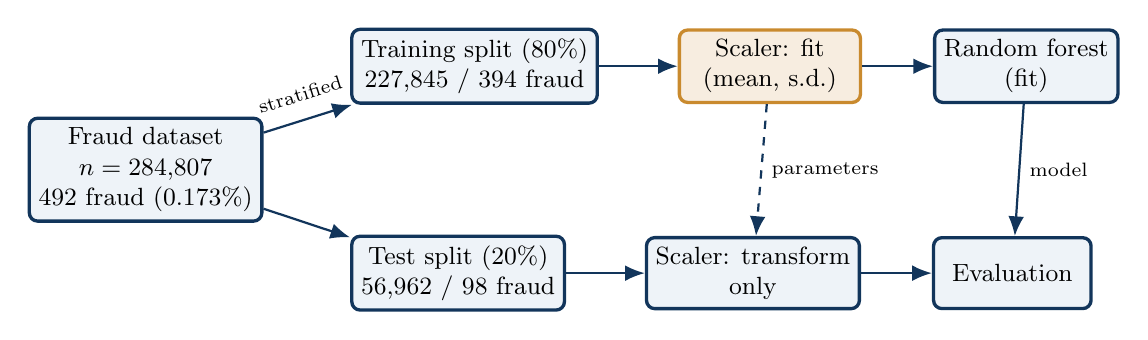
\begin{tikzpicture}[node distance=0.55cm and 0.7cm, font=\footnotesize]
\node[flowbox, minimum width=2.6cm] (d) {Fraud dataset\\$n = 284{,}807$\\492 fraud (0.173\%)};
\node[flowbox, minimum width=2.6cm, above right=0.15cm and 1.1cm of d] (tr) {Training split (80\%)\\227{,}845 / 394 fraud};
\node[flowbox, minimum width=2.6cm, below right=0.15cm and 1.1cm of d] (te) {Test split (20\%)\\56{,}962 / 98 fraud};
\node[accentbox, minimum width=2.3cm, right=1.0cm of tr] (sc) {Scaler: fit\\(mean, s.d.)};
\node[flowbox, minimum width=2.3cm, right=1.0cm of te] (st) {Scaler: transform\\only};
\node[flowbox, minimum width=2.0cm, right=0.9cm of sc] (m) {Random forest\\(fit)};
\node[flowbox, minimum width=2.0cm, right=0.9cm of st] (ev) {Evaluation};
\draw[arrow] (d) -- node[above=3pt, sloped, pos=0.5, font=\scriptsize] {stratified} (tr);
\draw[arrow] (d) -- (te);
\draw[arrow] (tr) -- (sc); \draw[arrow] (te) -- (st);
\draw[arrow] (sc) -- (m); \draw[arrow] (st) -- (ev);
\draw[arrow, dashed] (sc) -- node[right, font=\scriptsize] {parameters} (st);
\draw[arrow] (m) -- node[right, font=\scriptsize] {model} (ev);
\end{tikzpicture}
\vspace{0.6em}
\begin{itemize}\footnotesize
\item From \texttt{streamlit/modeling.py}; \texttt{notebooks/Class6\_Model\_Training\_.ipynb} applies the same pattern to the Iris dataset.
\item \textbf{Stratification} keeps the fraud rate at 0.173\% in both splits (394 and 98 positive samples); a random split could leave the test set with noticeably fewer or more positives.
\item \textbf{The scaler is fitted on the training split only} and then applied to the test split with the same parameters, to avoid preprocessing leakage (Class 13).
\end{itemize}
\coursefooter
\end{frame}

\begin{frame}{Experimentation is an engineering discipline}
\begin{itemize}
\item The purpose of experimentation is not to accumulate scores, but to support a credible model choice.
\item Every run should answer a stated question: does a new feature, a different model family, or additional tuning justify its complexity?
\item The evaluation protocol and the minimum improvement considered meaningful must be fixed before results are inspected.
\item Without a stated question, an experiment tracker stores results without providing evidence.
\end{itemize}
\coursefooter
\end{frame}

\begin{frame}{What must be tracked, and why}
\begin{tabularx}{\textwidth}{>{\bfseries}l X}
Dataset version or extraction date & Allows a result to be reproduced on the same data. \\
\addlinespace[0.3em]
Feature pipeline version & Separates the effect of preprocessing changes from that of model changes. \\
\addlinespace[0.3em]
Hyperparameters and random seeds & Identify the exact configuration that produced a result. \\
\addlinespace[0.3em]
Metrics, confusion matrices, artifacts & Allow the trained model, not only a number, to be audited. \\
\addlinespace[0.3em]
Code commit or notebook snapshot & Allows the logic behind a run to be replayed later (Class 17). \\
\bottomrule
\end{tabularx}
\coursefooter
\end{frame}

\begin{frame}{Fair comparison and sources of bias}
\begin{columns}[T]
\column{0.48\textwidth}
\textbf{A fair comparison uses}
\begin{itemize}
\item the same data split or validation protocol;
\item the same preprocessing, unless preprocessing is the object of the experiment;
\item metrics chosen for the actual decision;
\item a measure of variability, e.g.\ mean $\pm$ standard deviation across cross-validation folds.
\end{itemize}
\column{0.48\textwidth}
\textbf{Bias is introduced by}
\begin{itemize}
\item reusing the test set until it becomes part of tuning (model-selection leakage);
\item hidden notebook state and untracked edits;
\item reporting only the best run.
\end{itemize}
\end{columns}
\coursefooter
\end{frame}

\begin{frame}{Hyperparameter search strategies}
\begin{tabularx}{\textwidth}{>{\bfseries}l X}
Manual tuning & Small problems; useful to build intuition. \\
\addlinespace[0.3em]
Grid search & Exhaustive evaluation of a small, structured search space. \\
\addlinespace[0.3em]
Random search & Better coverage when only a few of many hyperparameters matter (Bergstra and Bengio, 2012). \\
\addlinespace[0.3em]
Bayesian optimization & A surrogate model of the score guides the search; suited to expensive models. \\
\bottomrule
\end{tabularx}
\vspace{0.6em}
\begin{itemize}
\item A tuned model should outperform a simple, default, or previously deployed baseline by more than the variability of the estimate.
\end{itemize}
\coursefooter
\end{frame}

\begin{frame}{Neptune example: search space and protocol}
\begin{columns}[T]
\column{0.5\textwidth}
\begingroup\footnotesize
\textbf{Search space} of a gradient boosting regressor:
\vspace{0.3em}

\begin{tabular}{>{\ttfamily}l l}
\normalfont\bfseries Hyperparameter & \bfseries Values \\
\toprule
n\_estimators & 100, 200, 300 \\
max\_depth & 3, 5, 7 \\
learning\_rate & 0.05, 0.1, 0.2 \\
min\_samples\_split & 2, 5, 10 \\
\bottomrule
\end{tabular}
\par\endgroup
\column{0.48\textwidth}
\begingroup\footnotesize
\textbf{Protocol:}
\begin{itemize}
\item Data: red wine quality, 1{,}599 samples; target \texttt{quality}.
\item Split: 75\% training, 25\% test (fixed seed).
\item Grid search: $3^4 = 81$ configurations $\times$ 5-fold cross-validation $=$ 405 fits, scored by $R^2$ on the training split.
\item The test split is used once, after selection.
\end{itemize}
\par\endgroup
\end{columns}
\vspace{0.6em}
{\scriptsize From \texttt{notebooks/Class7\_Model\_Tuning\_Neptune.ipynb}, which combines \texttt{GridSearchCV} with the Neptune experiment tracker.\par}
\coursefooter
\end{frame}

\begin{frame}{Neptune example: a tracked run record}
\begingroup\footnotesize
Every run stores its configuration, results, and artifacts together, in the same place, automatically:
\par\endgroup
\vspace{0.4em}
\centering
\begingroup\footnotesize
\renewcommand{\arraystretch}{1.2}
\begin{tabularx}{0.9\textwidth}{>{\ttfamily}l X}
\normalfont\bfseries Field & \bfseries Value logged by the notebook \\
\toprule
best/parameters & learning\_rate $= 0.05$, max\_depth $= 7$, min\_samples\_split $= 5$, n\_estimators $= 200$ \\
best/cv\_score & mean $R^2$ over the 5 folds of the selected configuration \\
test/mse & 0.349 \\
test/r2 & 0.436 \\
artifacts/model & \texttt{best\_gb\_model.pkl} (serialized estimator) \\
\bottomrule
\end{tabularx}
\par\endgroup
\vspace{0.5em}
\begin{itemize}\footnotesize
\item Mean squared error (MSE) and coefficient of determination ($R^2$) are computed once on the test split, after selection.
\item The pattern is tool-independent: MLflow, Weights \& Biases, or an internal registry store the same record. The serialized artifact is the bridge to deployment (Class 30).
\end{itemize}
\coursefooter
\end{frame}

\begin{frame}{From a notebook run to a governed asset}
\centering
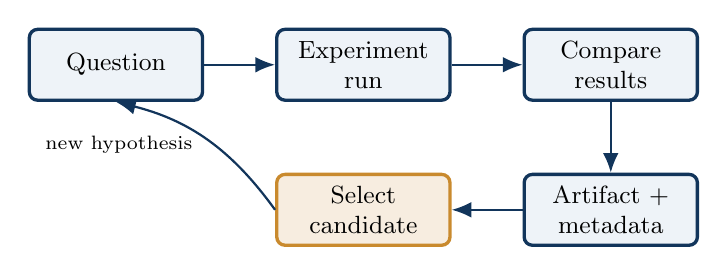
\begin{tikzpicture}[node distance=0.9cm and 0.9cm]
\node[flowbox] (question) {Question};
\node[flowbox, right=of question] (run) {Experiment\\run};
\node[flowbox, right=of run] (compare) {Compare\\results};
\node[flowbox, below=of compare] (artifact) {Artifact +\\metadata};
\node[accentbox, left=of artifact] (select) {Select\\candidate};
\draw[arrow] (question) -- (run);
\draw[arrow] (run) -- (compare);
\draw[arrow] (compare) -- (artifact);
\draw[arrow] (artifact) -- (select);
\draw[arrow, bend right=20] (select.west) to node[left=4pt, pos=0.45, font=\scriptsize] {new hypothesis} (question.south);
\end{tikzpicture}
\coursefooter
\end{frame}

\begin{frame}{Common tuning mistakes}
\begin{itemize}
\item Tuning hyperparameters on the test set.
\item Comparing runs trained with different preprocessing.
\item Reporting only the best score, without its variability or computational cost.
\item Ignoring that a slightly less accurate model may be considerably easier to deploy, explain, or monitor.
\end{itemize}
\coursefooter
\end{frame}

\begin{frame}{Evaluation metrics must match the task}
\begin{itemize}
\item Tracking identifies which run performed best; it does not establish whether that run is adequate for the decision it supports.
\item \textbf{Imbalanced classification:} with true and false positives and negatives (TP, FP, TN, FN),
\[
\text{precision} = \frac{TP}{TP + FP}, \qquad \text{recall} = \frac{TP}{TP + FN},
\]
summarized over all thresholds by the area under the precision--recall curve (PR-AUC); accuracy alone is misleading.
\item \textbf{Regression:} mean absolute error (MAE) and root mean squared error (RMSE), expressed in the unit that matters operationally.
\item \textbf{Calibration:} required whenever a downstream action depends on the predicted probability rather than only on the predicted class.
\end{itemize}
\coursefooter
\end{frame}

\begin{frame}{The fraud dataset at a glance}
\centering
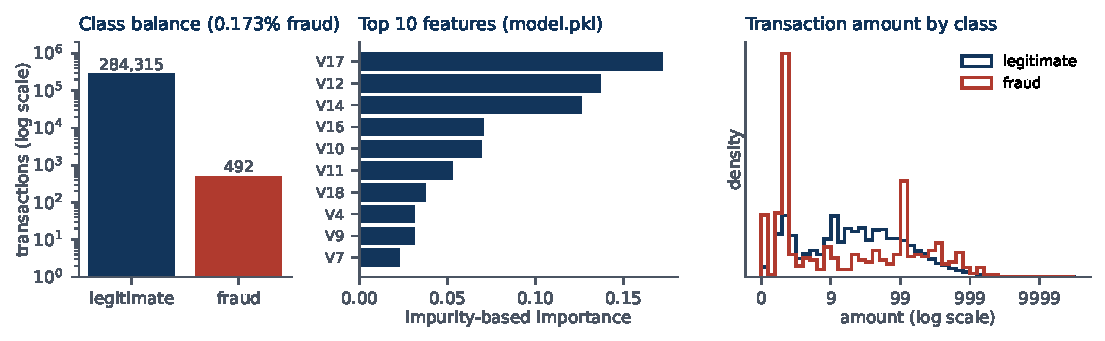
\includegraphics[width=\textwidth,height=0.46\textheight,keepaspectratio]{images/class18_fraud_overview.pdf}

\vspace{0.3em}
\begin{itemize}\footnotesize
\item \textbf{Imbalance:} 492 of 284{,}807 transactions (0.173\%) are fraudulent; the first difficulty is the rarity of the positive class, not the choice of algorithm.
\item \textbf{Importance:} three principal components (\texttt{V17}, \texttt{V12}, \texttt{V14}) account for 43\% of the impurity-based importance of the deployed random forest; importance measures association, not causal effect.
\item \textbf{Skewness:} amounts span four orders of magnitude, and fraudulent transactions tend to be smaller (median 9.25 versus 22.00); scaling, evaluation, and threshold choice interact with this shape.
\end{itemize}
\coursefooter
\end{frame}

\begin{frame}{Repository example: inspecting the errors}
\begin{columns}[T]
\column{0.42\textwidth}
\centering
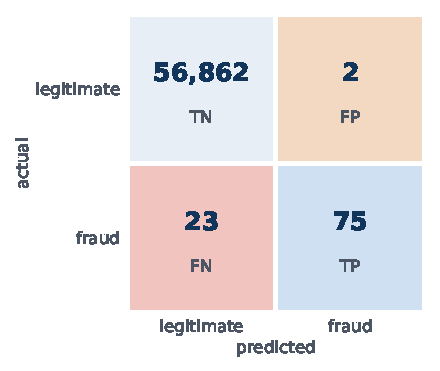
\includegraphics[width=0.95\linewidth]{images/class18_confusion_matrix.pdf}

{\scriptsize Test split (56{,}962 transactions), best random forest of the grid search in \texttt{Credit\_Card\_Fraud\_Detection\_Solution.ipynb}.\par}
\column{0.56\textwidth}
\begingroup\footnotesize
\[
\text{precision} = \frac{75}{75 + 2} = 0.97, \qquad \text{recall} = \frac{75}{75 + 23} = 0.77
\]
\[
\text{accuracy} = \frac{56{,}862 + 75}{56{,}962} = 0.9996
\]
\par\endgroup
\begin{itemize}\footnotesize
\item 23 of the 98 fraudulent transactions are missed (FN), while only 2 legitimate ones are flagged (FP).
\item Accuracy, at 99.96\%, conceals both numbers; the confusion matrix exposes them directly.
\item Whether 23 missed frauds are acceptable depends on the cost of a missed fraud relative to a false alarm, which motivates the threshold analysis that follows.
\end{itemize}
\end{columns}
\coursefooter
\end{frame}

\begin{frame}{Why accuracy fails under class imbalance}
\begin{block}{Fraud example}
With 0.173\% fraudulent transactions, a classifier that always predicts ``legitimate'' attains an accuracy of 99.83\%, a recall of 0, and no operational value.
\end{block}
\begin{itemize}
\item Precision, recall, and the decision threshold are therefore part of the engineering design, not a post-hoc check.
\end{itemize}
\coursefooter
\end{frame}

\begin{frame}{A model creates value only through an interface}
\begin{itemize}
\item A trained model that cannot be invoked or interpreted has limited practical value, regardless of its offline metrics.
\item An interface makes predictions available to users, services, and operational workflows.
\item The interface also determines trust: input validation, response format, and clarity matter as much as the metric used to select the model.
\end{itemize}
\coursefooter
\end{frame}

\begin{frame}{A prediction is not a decision}
\begin{itemize}
\item A fraud score suggests escalation, not guilt; a process alert suggests investigation, not automatic shutdown.
\item A classifier outputs an estimate $\hat{p}(\mathbf{x})$ of $P(y = 1 \mid \mathbf{x})$; the decision rule is $\hat{y} = \mathbf{1}[\hat{p}(\mathbf{x}) \ge \tau]$.
\item If $\hat{p}$ is calibrated and $c_{FP}$, $c_{FN}$ denote the costs of a false positive and a false negative, the expected cost is minimized by
\[
\tau^{*} = \frac{c_{FP}}{c_{FP} + c_{FN}}.
\]
\end{itemize}
\begin{block}{Engineering implication}
The threshold that turns a probability into a decision is a design choice derived from costs, not a by-product of the model (the default $\tau = 0.5$ assumes $c_{FP} = c_{FN}$).
\end{block}
\coursefooter
\end{frame}

\begin{frame}{Choosing the threshold: a cost analysis}
\centering
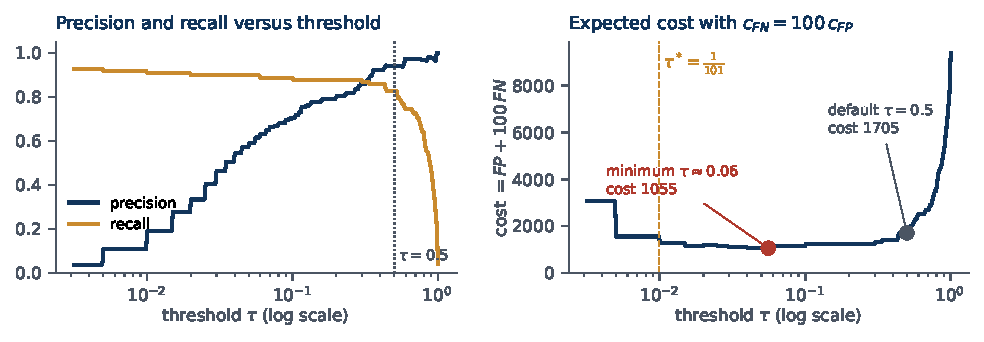
\includegraphics[width=\textwidth,height=0.4\textheight,keepaspectratio]{images/class18_threshold_cost.pdf}

\vspace{0.2em}
\begin{itemize}\footnotesize
\item Deployed model (\texttt{streamlit/model.pkl}) on the test split, assuming a missed fraud costs 100 times a false alarm.
\item \textbf{Default} $\tau = 0.5$: 81 frauds detected, 17 missed, 5 false alarms; cost 1{,}705. \textbf{Minimum} at $\tau \approx 0.06$: 88 detected, 10 missed, 55 false alarms; cost 1{,}055 ($-38\%$).
\item The theoretical $\tau^{*} = 1/101 \approx 0.01$ differs from the empirical minimum because random-forest scores (vote fractions) are not calibrated probabilities.
\item In practice, $\tau$ must be chosen on a validation split; selecting it on the test split, as in this illustration, is model-selection leakage.
\end{itemize}
\coursefooter
\end{frame}

\begin{frame}{Repository example: decision support in Streamlit}
\centering
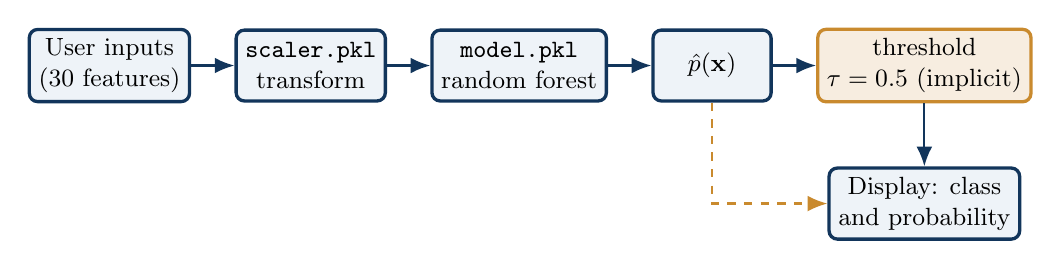
\begin{tikzpicture}[node distance=0.55cm, font=\footnotesize]
\node[flowbox, minimum width=1.9cm] (in) {User inputs\\(30 features)};
\node[flowbox, minimum width=1.7cm, right=of in] (sc) {\texttt{scaler.pkl}\\transform};
\node[flowbox, minimum width=1.7cm, right=of sc] (m) {\texttt{model.pkl}\\random forest};
\node[flowbox, minimum width=1.5cm, right=of m] (p) {$\hat{p}(\mathbf{x})$};
\node[accentbox, minimum width=1.9cm, right=of p] (t) {threshold\\$\tau = 0.5$ (implicit)};
\node[flowbox, minimum width=1.9cm, below=0.8cm of t] (out) {Display: class\\and probability};
\draw[arrow] (in) -- (sc); \draw[arrow] (sc) -- (m); \draw[arrow] (m) -- (p); \draw[arrow] (p) -- (t); \draw[arrow] (t) -- (out);
\draw[arrow, dashed, coursegold] (p.south) |- (out.west);
\end{tikzpicture}
\vspace{0.6em}
\begin{itemize}\footnotesize
\item From \texttt{streamlit/pages/App\_Credit\_Card.py}: the interface shows both the predicted class and the estimated probability.
\item The class comes from \texttt{model.predict}, i.e.\ the implicit threshold $\tau = 0.5$; under the cost assumption of the previous analysis, a threshold near 0.06 would detect 7 more frauds in the test split.
\item The threshold should be an explicit, documented, and versioned parameter of the interface, not a default of the library.
\end{itemize}
\coursefooter
\end{frame}

\begin{frame}{Requirements for a decision-support dashboard}
\begin{itemize}
\item An explicit statement of what the model does and does not do.
\item Inputs that correspond to meaningful domain variables rather than technical internals.
\item Outputs that support action: alert, score, trend, or explanation.
\item References to data provenance, model version, and monitoring signals.
\end{itemize}
\coursefooter
\end{frame}

\begin{frame}{Where trust breaks down}
\begin{itemize}
\item The interface conceals uncertainty behind a single, apparently precise number.
\item The inputs presented to users do not match the assumptions under which the model was trained.
\item The threshold was chosen once, informally, and never revisited as the data changed.
\item The dashboard makes a demonstration model appear authoritative although it has not been validated for that purpose.
\end{itemize}
\coursefooter
\end{frame}

\begin{frame}{Repository connections}
\repoactivity{
\begin{itemize}
\item \texttt{notebooks/Class6\_Model\_Training\_.ipynb}: baseline split, tuning, evaluation, and serialization (Iris dataset).
\item \texttt{notebooks/Class7\_Model\_Tuning\_Neptune.ipynb}: grid search with Neptune tracking (wine quality regression).
\item \texttt{Credit\_Card\_Fraud\_Detection\_Solution.ipynb}: evaluation of the fraud classifier.
\item \texttt{streamlit/modeling.py} and \texttt{streamlit/pages/App\_Credit\_Card.py}: training, persistence of model and scaler, and the human-facing decision interface.
\end{itemize}
}
\coursefooter
\end{frame}

\begin{frame}{Papers and materials}
\readinglist{
\fontsize{6.8}{8.2}\selectfont
\begin{columns}[T]
\column{0.5\textwidth}
\begin{itemize}\setlength{\itemsep}{1pt}
\item Bergstra, J., Bengio, Y. (2012). Random search for hyper-parameter optimization. \emph{Journal of Machine Learning Research}, 13, 281--305.
\item Bergstra, J., Yamins, D., Cox, D. (2013). Making a science of model search: Hyperparameter optimization in hundreds of dimensions for vision architectures. \emph{Proceedings of ICML}, PMLR 28(1), 115--123.
\item Elkan, C. (2001). The foundations of cost-sensitive learning. \emph{Proceedings of IJCAI}, 973--978.
\item Saito, T., Rehmsmeier, M. (2015). The precision-recall plot is more informative than the ROC plot when evaluating binary classifiers on imbalanced datasets. \emph{PLoS ONE}, 10(3), e0118432.
\item Niculescu-Mizil, A., Caruana, R. (2005). Predicting good probabilities with supervised learning. \emph{Proceedings of ICML}, 625--632.
\end{itemize}
\column{0.5\textwidth}
\begin{itemize}\setlength{\itemsep}{1pt}
\item Domingos, P. (2012). A few useful things to know about machine learning. \emph{Communications of the ACM}, 55(10), 78--87.
\item Huyen, C. (2022). \emph{Designing Machine Learning Systems}. O'Reilly.
\item scikit-learn User Guide: \href{https://scikit-learn.org/stable/modules/grid_search.html}{tuning hyperparameters}; \href{https://scikit-learn.org/stable/modules/model_evaluation.html}{model evaluation}.
\item Tool documentation: \href{https://docs.neptune.ai/}{Neptune}; \href{https://mlflow.org/docs/latest/index.html}{MLflow}; \href{https://docs.streamlit.io/}{Streamlit}.
\end{itemize}
\end{columns}
}
\coursefooter
\end{frame}

\begin{frame}{Take-away message}
\vfill
\centering
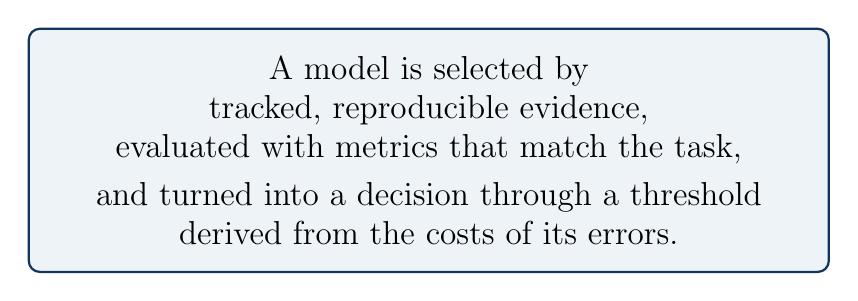
\begin{tikzpicture}
\node[fill=courseice, draw=courseblue, thick, rounded corners=4pt, inner sep=10pt, text width=0.78\textwidth, align=center, font=\large] {A model is selected by tracked, reproducible evidence,\\ evaluated with metrics that match the task,\\[0.3em] and turned into a decision through a threshold\\ derived from the costs of its errors.};
\end{tikzpicture}

\vfill
{\Large\bfseries\color{courseblue} Thank you for your attention.}

\vspace{0.4em}
{\small\color{coursegray} Next: Class 19 --- online machine learning and concept drift.}
\vfill
\coursefooter
\end{frame}

\end{document}
